% !TEX program = pdflatex

\documentclass[a4paper,10pt]{article}
\usepackage[utf8]{inputenc}
\usepackage{amsmath}
\usepackage{amssymb}
\usepackage{graphicx}
\usepackage{float}
\usepackage{pgfplots}
\pgfplotsset{compat=newest}
\usepackage{cite}
\usepackage{coffee4}
\usepackage{trollface}

\usepackage{ClearSans}
\usepackage[T1]{fontenc}
\usepackage{tikz}
%
\usetikzlibrary{fit,backgrounds}
%
\def\gamefont{\bfseries\sffamily}
%
\definecolor{grid color}{HTML}{BBADA0}
\definecolor{pixel 0}{HTML}{CCC0B3}
\definecolor{pixel 2}{HTML}{EEE4DA}
\definecolor{pixel 4}{HTML}{EDE0C8}
\definecolor{pixel 8}{HTML}{F2B179}
\definecolor{pixel 16}{HTML}{F59563}
\definecolor{pixel 32}{HTML}{F67C5F}
\definecolor{pixel 64}{HTML}{F65E3B}
\definecolor{pixel 128}{HTML}{EDCF72}
\definecolor{pixel 256}{HTML}{EDCC61}
\definecolor{pixel 512}{HTML}{EDC850}
\definecolor{pixel 1024}{HTML}{EDC53F}
\definecolor{pixel 2048}{HTML}{EDC22E}
\definecolor{pixel 4096}{HTML}{3E3933}
%
\definecolor{small color}{HTML}{776E65}
\definecolor{big color}{HTML}{F9F6F2}
%
\tikzset{
  case 2048 base/.style={
    minimum size=9mm,rounded corners=.3mm,text=#1,inner sep=0,line width=0,
  },
  %
  case 2048 Large/.style={font=\Large\gamefont,case 2048 base=#1},
  case 2048 large/.style={font=\large\gamefont,case 2048 base=#1},
  case 2048 normal/.style={font=\normalsize\gamefont,case 2048 base=#1},
  %
  case 2048 0/.style={case 2048 Large=black,fill=pixel 0,node contents={}},
  case 2048 2/.style={case 2048 Large=small color,fill=pixel 2,node contents={2}},
  case 2048 4/.style={case 2048 Large=small color,fill=pixel 4,node contents={4}},
  case 2048 8/.style={case 2048 Large=big color,fill=pixel 8,node contents={8}},
  case 2048 16/.style={case 2048 Large=big color,fill=pixel 16,node contents={16}},
  case 2048 32/.style={case 2048 Large=big color,fill=pixel 32,node contents={32}},
  case 2048 64/.style={case 2048 Large=big color,fill=pixel 64,node contents={64}},
  case 2048 128/.style={case 2048 large=big color,fill=pixel 128,node contents={128}},
  case 2048 256/.style={case 2048 large=big color,fill=pixel 256,node contents={256}},
  case 2048 512/.style={case 2048 large=big color,fill=pixel 512,node contents={512}},
  case 2048 1024/.style={case 2048 normal=big color,fill=pixel 1024,node contents={1024}},
  case 2048 2048/.style={case 2048 normal=big color,fill=pixel 2048,node contents={2048}},
  case 2048 4096/.style={case 2048 normal=big color,fill=pixel 4096,node contents={4096}},
}




%opening
\title{A test of the sharelatex compiler}
\author{Bas Rustenburg}

\begin{document}

\maketitle

\begin{abstract}
Lorem ipsum dolor sit amet, ridens consequuntur ut sit, an has suas modus cetero.
Pri cibo definitionem ne, graeco splendide vel et, vel ne dolorum laoreet. \cite{rasbastenburg2014}
Eum ex oratio dolorum meliore, suas dignissim abhorreant in vel.
Similique assueverit concludaturque te vix, everti sententiae ne nec.
Noster maiorum insolens an sea, te possit diceret voluptatibus sea, ad pri ludus ridens.
Est no quas nostrum maluisset, cu quas adhuc salutandi vix.
\end{abstract}



\section{Section 1}
Et sea impedit fierent tincidunt, nec delenit definitiones delicatissimi et.
Velit choro rationibus ad nec.

\begin{figure}[H]
 \centering
 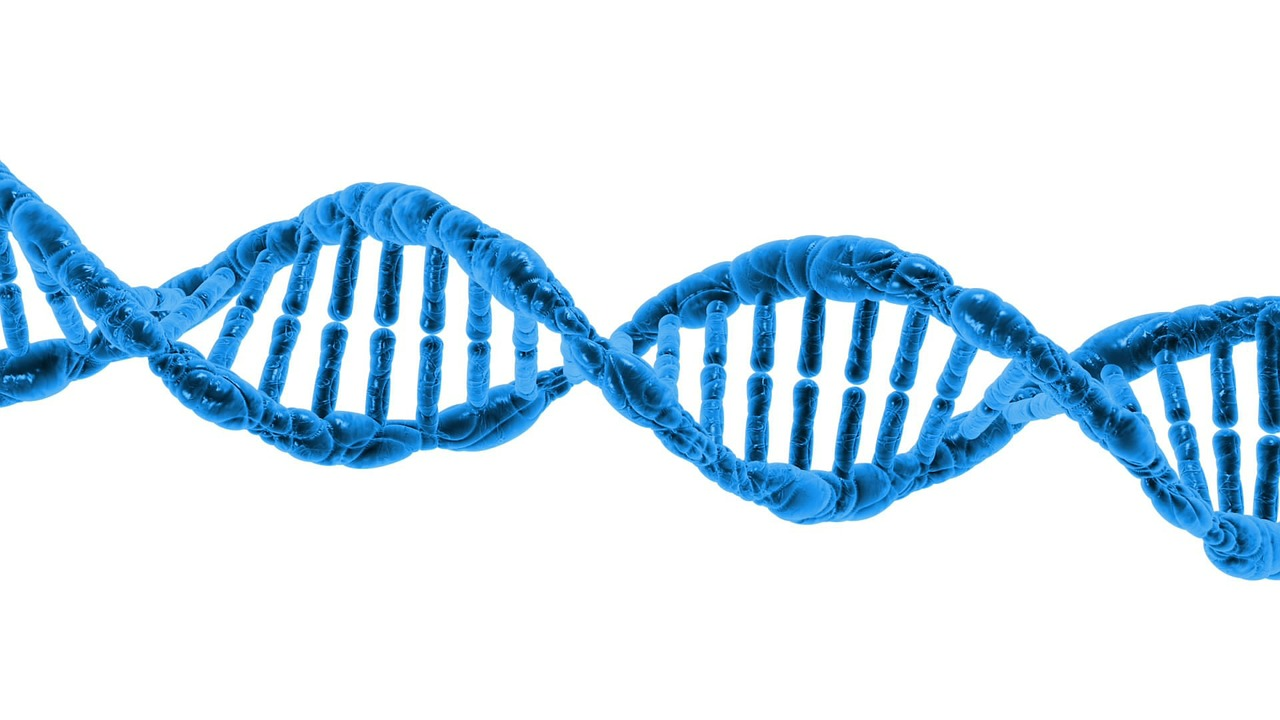
\includegraphics[width=\textwidth,keepaspectratio=true]{./dna.jpg}
 % dna.jpg: 1280x720 pixel, 72dpi, 45.16x25.40 cm, bb=0 0 1280 720
 \caption{Iudicabit eloquentiam vim te, nihil splendide sit ne.}
 \label{fig:dna}
\end{figure}

In eum natum insolens, ex sit dicant nonumy reprehendunt.
Saepe epicurei mea at, mea everti fuisset accusam et.
Detraxit menandri ex vis, sed id quas nonumes officiis, cu verear reprimique scribentur vis.
Ad his malorum phaedrum dissentiet.

\cofeAm{0.1}{1}{0}{0}{0}

Ipsum mentitum id usu, qui eu nisl harum.
No epicurei forensibus vel.
Sit nulla nihil urbanitas no.
Et erant suscipit definitionem his, platonem iudicabit ei pro.



Atqui prodesset no nec, putant aperiam te vel.
At laudem animal duo, homero melius torquatos est ei.
At quaestio argumentum eos.
Mazim vocibus assentior no duo, an singulis temporibus sed, mei eu veri officiis maiestatis.
Quis possit inermis mel in, est esse lobortis ei.

\begin{align}
A_1&=N_0(\lambda;\Omega')-\phi(\lambda;\Omega'), \twoheadleftarrow \\
A_2&=\phi(\lambda;\Omega')-\phi(\lambda;\Omega),\\
\intertext{et}A_3&=\mathcal{N}(\lambda;\omega).
\end{align}

Natum suscipit no pro, nominati perpetua accommodare has an, te vel atqui postea labore. Agam salutandi eum id, eam inani essent cu. Et graece cotidieque est. Vix ut sapientem voluptatum elaboraret, ad sit essent qualisque. No quot imperdiet mel. Qui tritani corrumpit ea.
\begin{center}
 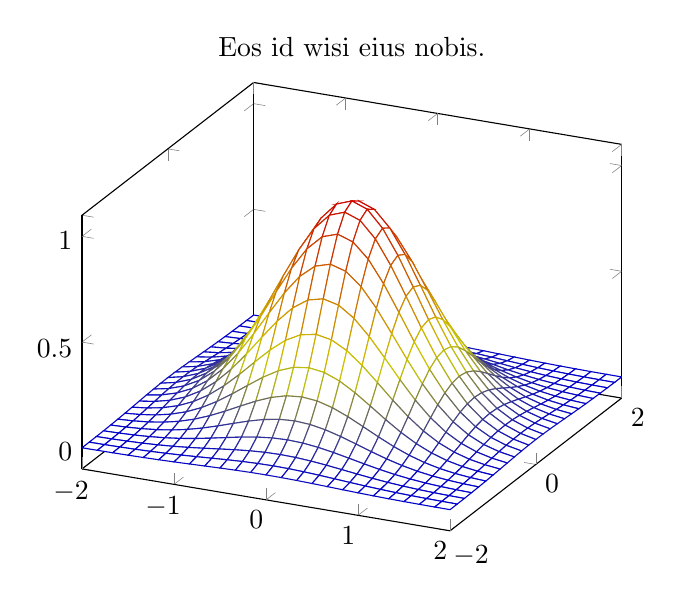
\begin{tikzpicture}
\centering
	\begin{axis}[title=Eos id wisi eius nobis.]
	\addplot3[surf,fill=white,domain=-2:2] {exp(-x^2-y^2)};	
	\end{axis}
\end{tikzpicture}

\end{center}


Illum altera tamquam qui eu, usu ad detraxit dissentiunt. Vis zril tincidunt disputationi no. Cum eu dictas consequat. In senserit dissentias vim. Graecis invenire te qui, et virtute tacimates philosophia mea.

No quando nemore eos, cum idque menandri assentior ea, eu mel natum elitr percipit. Modo mollis forensibus duo ei. Ea assum dolorum vulputate eum. Ea eirmod offendit duo. Ex nec probatus recusabo accusamus, ei mel falli graeci.

\begin{center}
 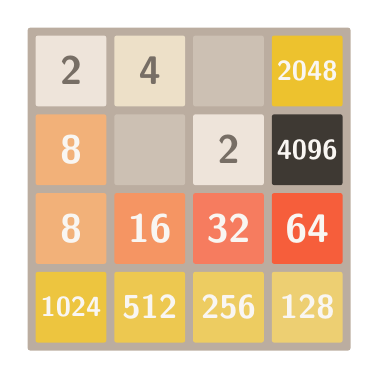
\begin{tikzpicture}
  \def\pixels{
    {2,4,0,2048},
    {8,0,2,4096},
    {8,16,32,64},
    {1024,512,256,128},
  }

  \foreach \line [count=\y] in \pixels {
    \foreach \pix [count=\x] in \line {
      \path (\x,-\y) node[name=c2048-\x-\y,case 2048 \pix];
    }
  }

  \begin{scope}[on background layer]
    \node[fill=grid color,fit=(c2048-1-1)(c2048-4-4),
    inner sep=1mm,rounded corners=.3mm]{};
  \end{scope}
\end{tikzpicture}

\end{center}


Vis homero convenire ex, nam imperdiet instructior no. Homo sapiens non urinat in ventum. Eam ea debitis ullamcorper, nisl noluisse nam ad. Sit copiosae assentior no, nam an amet ocurreret. At legere nostro sit, est nonumy partiendo cu, vel eu platonem recteque.

\bibliography{article}{}
\bibliographystyle{plain}

{\small \trollface}

\end{document}
